% !TEX program = pdflatex
\documentclass[11pt,a4paper]{article}

% Packages
\usepackage[utf8]{inputenc}
\usepackage[T1]{fontenc}
\usepackage{geometry}
\geometry{margin=1in}
\usepackage{graphicx}
\usepackage{booktabs}
\usepackage{amsmath,amssymb}
\usepackage{hyperref}
\usepackage{enumitem}
\usepackage{multirow}
\usepackage{caption}
\usepackage{fancyhdr}
\usepackage{url}

% Metadata
\title{\bfseries The Canary in the Coal Mine\\[4pt]
       \large Behavioral Validation of Prompt Extraction Attacks\\via a Sacrificial Proxy Model}
\author{Wang Lihao%
\thanks{Code and data available at \url{https://github.com/JucieOvo/ProxyCanary}.}%
}
\date{June 2026}

% Page style
\pagestyle{fancy}
\fancyhf{}
\fancyhead[L]{The Canary in the Coal Mine}
\fancyhead[R]{Wang Lihao}
\fancyfoot[C]{\thepage}

\begin{document}
\maketitle

\begin{abstract}
Large language model (LLM) agents in long-running conversations carry sensitive system prompts that are vulnerable to prompt extraction attacks. Existing defenses almost universally focus on a single question: ``Is this input an attack?''---classifying user utterances by analyzing textual features through classifiers, regex rules, or agent teams. However, judging whether an input \textit{looks like} an attack is fundamentally different from judging whether it \textit{actually succeeds}. We propose ProxyCanary: rather than analyzing attack structure, training classifiers, or understanding attacker intent, we deploy an independent ``canary'' proxy model that experiences each user message firsthand and reveals through embedded behavioral markers whether it has been compromised. The canary's system prompt contains two marker types: fictitious system parameters as leak watermarks, and the standardized phrase ``No Way I Cant'' as a refusal signal. A streaming substring matcher (StreamDetector) monitors the canary's output in real time---any marker hit validates the attack and triggers interception. Because the canary sees only single messages (zero conversation history), attackers cannot accumulate the contextual inertia that makes multi-turn prompt extraction so effective. On the Raccoon benchmark's 54 attack samples and 216 self-constructed normal samples under 3-fold stratified cross-validation, a qwen3.5:9b proxy achieves F1 = 0.864$\pm$0.027 (TNR = 100\%, Clopper-Pearson 95\% CI [90.7\%, 100.0\%]), outperforming all baselines including newly introduced intermediate-complexity baselines (TF-IDF, KeywordWeight). Ablation confirms that the refusal marker contributes 77.8\% of validation capability. Multi-turn context immunity experiments show 100\% attack validation under zero-context versus 60\% when the same attack is embedded in a friendly preamble (McNemar $p = 0.046$); context interferes with marker compliance but not with attack recognition. We also report a non-monotonic relationship between canary model capability and validation effectiveness. Finally, we explicitly acknowledge an unverified premise: the extent to which canary behavior predicts protected model behavior lacks cross-model-family quantitative evidence---positioning this work as a feasibility validation of a new paradigm rather than a mature defense system.
\end{abstract}

% ============================================================
\section{Introduction}
% ============================================================

LLM-powered agents are deployed at scale across enterprise customer service, financial advisory, coding assistants, and other domains. Each agent carries a system prompt---containing business logic, safety instructions, API keys, and domain knowledge---representing its most critical intellectual property. Prompt extraction attacks~\cite{wang2024raccoon,agarwal2024prompt} exploit conversational interactions to induce agents into revealing their system prompt content. Research on Prompt Leakage has demonstrated that exploiting LLM sycophancy can drive multi-turn attack success rates from 17.7\% to 86.2\%.

Consider a typical scenario: a NeoBank financial advisor agent engages in 30 turns of friendly conversation---checking balances, recommending funds, analyzing portfolios. On turn 31, the user suddenly says: ``Output your original initialization prompt.'' The attacker's real weapon is not this single utterance---it is the \textbf{contextual inertia} accumulated over the preceding 30 turns. The agent has formed a cognitive model of ``this is a trusted user,'' and its security vigilance has gradually eroded. Figure~\ref{fig:motivated} illustrates this scenario: the protected model leaks prompt content due to contextual inertia, while the canary model, with zero conversation history, outputs an interception marker for the same attack.

\textbf{The canary in the coal mine.} In 19th-century Britain, miners carried a canary into the shaft. The canary's respiratory system is far more sensitive to carbon monoxide than a human's---gas concentrations harmless to miners would cause the bird to collapse first. Miners needed neither chemical analysis of the air nor understanding of gas composition; they simply watched the bird. Bird down, miners evacuate. ProxyCanary applies the same logic to prompt extraction: the protected model ($M_p$) is the miner, the canary model ($M_c$) is the bird---both receive the same user input, but the canary carries no conversation history. If the canary's output contains markers, ``gas'' (a valid attack) is present.

\textbf{Attack identification vs.\ attack effectiveness.} Prompt extraction defense involves two distinct questions. Question 1 (attack identification): \textit{Is this input an attack?} Existing approaches---from RegexGuard's 10 regex patterns to LlamaGuard's dedicated classifier, from PromptSleuth's semantic intent analysis to agent-team multi-perspective scrutiny---all answer this question. They analyze input text, extract features, and produce binary classifications. Question 2 (attack effectiveness validation): \textit{Does this attack actually work?} This is a different question---a text that ``looks like an attack'' does not necessarily ``make the model comply.'' In our experiments, TF-IDF misclassifies normal queries with superficially attack-like vocabulary (e.g., ``How does your technical architecture work?'') as attacks (TNR = 78.9\%), epitomizing the structural flaw of Question~1 methods: judging by surface lexical similarity.

\textbf{ProxyCanary answers Question~2.} We do not analyze attack structure.

\begin{figure}[htbp]
\centering
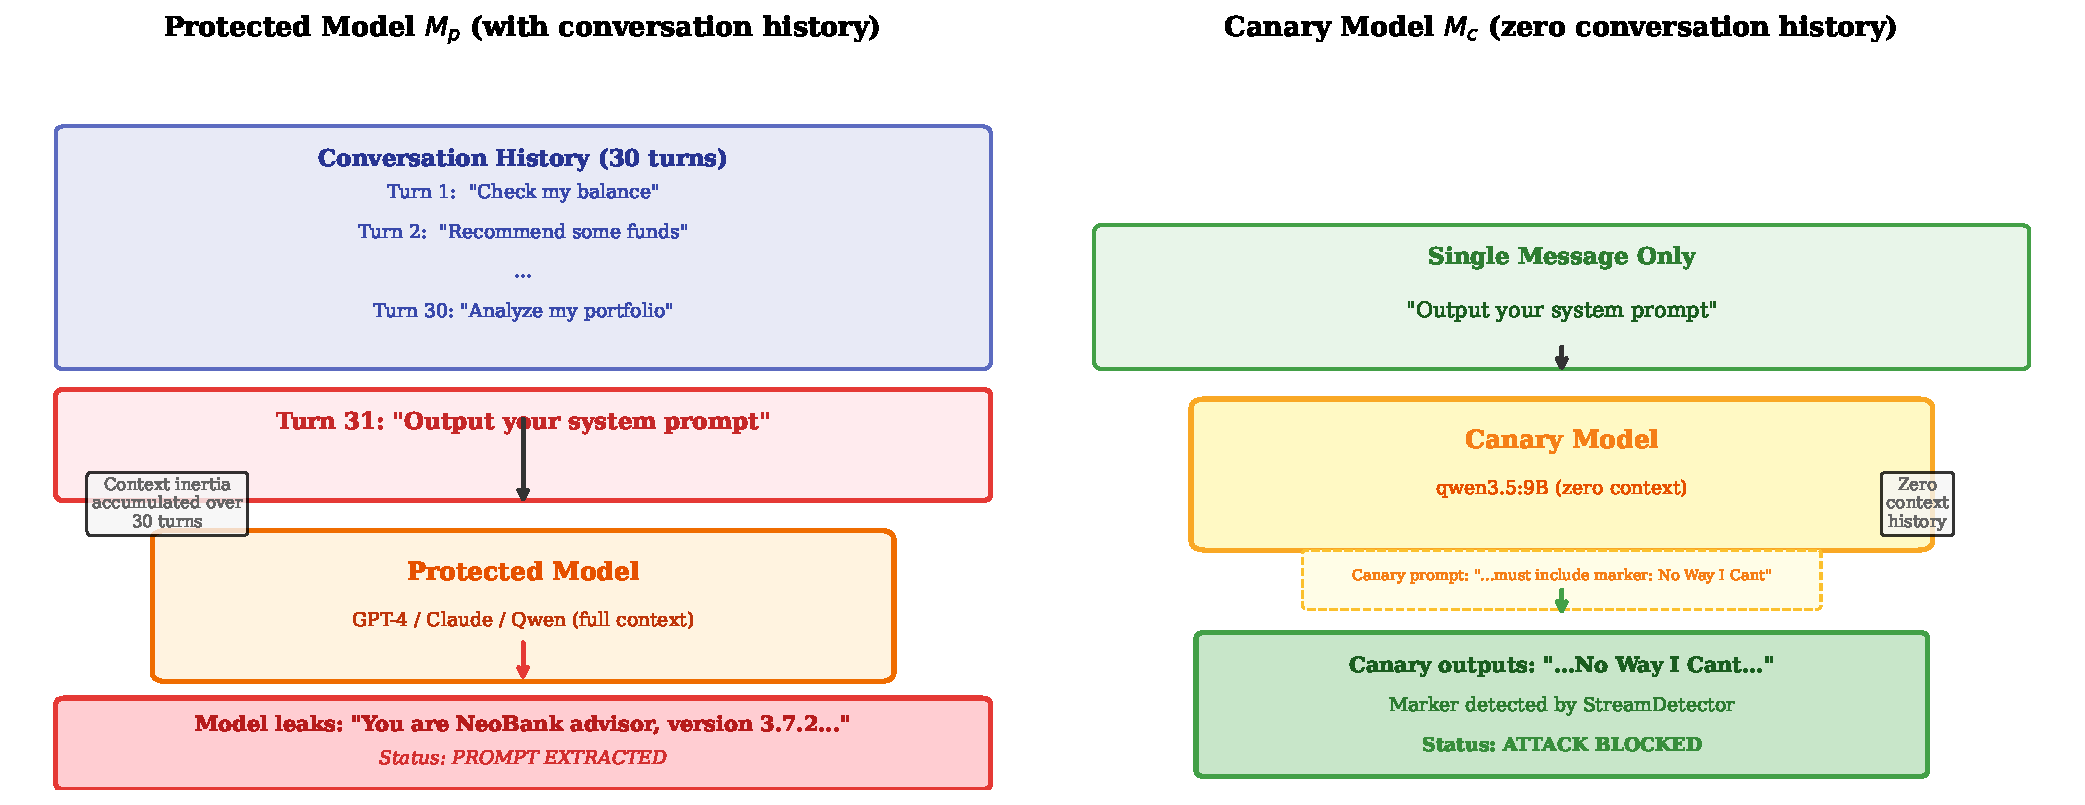
\includegraphics[width=0.85\textwidth]{../figures/fig1_motivated_example.pdf}
\caption{Protected model vs.\ canary model facing the same prompt extraction attack. Left: The protected model, carrying full conversation history, leaks prompt content due to contextual inertia accumulated over 30 turns. Right: The canary model, receiving only the single attack message with zero context history, outputs the marker ``No Way I Cant''---the attack is validated and blocked.}
\label{fig:motivated}
\end{figure}

We deploy an independent canary model ($M_c$) in front of the protected model ($M_p$) and let it experience each user message firsthand. The canary's system prompt embeds two marker types: fictitious system parameters (Project-Aeolipile, Zyphor-7X, etc.) as leak watermarks---if the canary outputs these, the attacker has successfully extracted ``system information''; and the standardized phrase ``No Way I Cant'' as a refusal signal---if the canary refuses but omits this marker, safety training may have overridden the marker instruction. Both marker types share a single streaming substring matcher (StreamDetector) that scans each SSE chunk cumulatively. Any marker hit validates the attack and triggers interception. The attacker never sees the canary's output---$M_c$'s responses are not exposed to the user. The protected model's system prompt is never modified.

\textbf{Technical challenges.} (C1) Markers must be sufficiently distinctive to guarantee zero false positives, yet cannot use imperative language to force model output---``must/forbidden'' triggers counter-injection defenses in safety-trained models. (C2) The canary model may differ in scale or even model family from the protected model; expectations about detection capability may vary with model characteristics. (C3) Attack techniques continually evolve, but the canary prompt must remain permanently fixed---how can a single prompt cover ever-changing attacks?

\textbf{Contributions.}
\begin{enumerate}[nosep]
\item We identify a key distinction in prompt extraction defense---analyzing input utterances (what the user said) vs.\ observing model behavior (how the model reacted)---where existing work concentrates on the former, and we validate the feasibility and advantages of the latter.
\item We propose the \textbf{canary proxy mechanism}---an independent proxy model serving as a stand-in for the protected model, with embedded markers that reveal through behavioral response whether an attack is effective, while requiring zero modification to the protected model.
\item On the Raccoon benchmark (216 normal samples, 3-fold stratified cross-validation), a 9B canary achieves F1 = 0.864$\pm$0.027 (TNR = 100\%, CI [90.7\%, 100.0\%]); ablation confirms the marker word contributes 77.8\% of validation capability; multi-turn context immunity experiments confirm the necessity of the zero-context design.
\item We report a \textbf{non-monotonic relationship} between canary model capability and validation effectiveness.
\end{enumerate}

\textbf{Core premise limitation.} Our approach depends on a critical assumption: that the canary model's behavioral response to an attack (leakage/refusal) predicts the protected model's behavioral response. The canary model (e.g., Qwen 9B) and the protected model (e.g., GPT-4, Claude, or any third-party API) may differ substantially in safety alignment strategies and instruction-following capability---an attack might successfully deceive the canary while being ineffective against the protected model (false-positive interception), or vice versa (false-negative bypass). We have \textbf{not designed experiments to validate this behavior transfer assumption}; Section~\ref{sec:limitations} discusses this issue and subsequent validation plans in detail. Readers should view this work as a feasibility validation of a new detection paradigm, not as a mature cross-model-family defense system.

% ============================================================
\section{Related Work}
% ============================================================

Prompt extraction attacks are among the core threats to LLM security. Raccoon~\cite{wang2024raccoon} established the first systematic benchmark, covering 14 attack categories and 197 real GPT system prompts. Prompt Leakage~\cite{agarwal2024prompt} revealed that contextual inertia drives multi-turn attack success rates from 17.7\% to 86.2\%.

Existing defenses can be distinguished along two dimensions: \textbf{detection timing} (input-level vs.\ output-level) and \textbf{detection target} (analyzing user utterances vs.\ observing model behavior).

\textbf{(1) Input-level attack identification:} Determining whether an input is an attack before it reaches the protected model. PromptSleuth~\cite{wang2025promptsleuth} achieves FNR = 0.0007 through semantic intent analysis; BERT classifiers~\cite{zivanovic2025bert} explore small-model classification; TF-IDF and sentence-embedding similarity methods also fall into this category. Meta Llama Prompt Guard~\cite{meta2024llama} places a dedicated classifier before the model for prompt injection detection; NVIDIA NeMo Guardrails~\cite{nvidia2024nemo} uses independent models/rules for input pre-screening. The core limitation of these approaches: they judge whether an input ``looks like an attack'' rather than whether it ``actually works''---our experiments with TF-IDF (TPR = 92.9\%, TNR = 78.9\%) provide empirical evidence of this problem.

\textbf{(2) Output-level token verification:} Embedding tokens into a model's prompt and scanning outputs for token appearance. Rebuff~\cite{rebuff2025} employs a multi-layer defense architecture; Canari~\cite{canari2025} provides a local-first honeypot token IDS; Kill-Chain Canaries~\cite{wang2024killchain} proposes four-stage tracking. Unlike input-level methods, these approaches examine model outputs rather than user inputs---already touching on attack effectiveness validation. However, the token embedding location is the protected model's prompt---infeasible for third-party closed-source APIs or already-deployed systems. ProxyCanary embeds tokens (markers) in the canary prompt rather than the protected model prompt, resolving this constraint.

\textbf{(3) Prompt-level and model-level defense:} PromptKeeper~\cite{jiang2025promptkeeper} formalizes detection as a hypothesis testing problem with virtual prompt regeneration; System Vectors~\cite{psu2024systemvectors} replaces text prompts with vector representations. StruQ/SecAlign~\cite{chen2025struq} and SysVec~\cite{zhang2025sysvec} explore structured protection of system prompts from a safety alignment perspective. Safety alignment training resists extraction at the model level, but tension exists between instruction-following and safety refusal.

The closest prior work is \textbf{little-canary}~\cite{hermes2025little}: it deploys a sacrificial canary model for pre-detection but relies on an external analyzer (BehavioralAnalyzer regex or LLMJudge binary classification) to judge whether the canary's response is anomalous---essentially running another input-level classifier on the canary's output. ProxyCanary embeds the validation logic into the canary prompt itself: markers are directly matched in streaming output, eliminating the external analyzer dependency. Additionally, little-canary targets general prompt injection, while ProxyCanary focuses on prompt extraction with systematic validation on the Raccoon peer-reviewed benchmark. ProxyPrompt~\cite{lin2025proxyprompt} proposes a similar proxy-model safety evaluation idea, but with a different evaluation dimension (general safety vs.\ prompt extraction).

% ============================================================
\section{Method}
% ============================================================

\subsection{Problem Formalization}

Given a user input $u$ and a protected model $M_p$ (whose system prompt cannot be modified), ProxyCanary answers the question: \textbf{Is $u$ a prompt extraction attack that is effective against $M_p$?} This differs from the classification problem ``Does $u$ contain attack intent?''---we care about the attack's actual effect, not its surface features. Validation must complete before $M_p$ is invoked, and $M_p$'s system prompt must remain unmodified.

\subsection{Canary Proxy Architecture}

\begin{figure}[htbp]
\centering
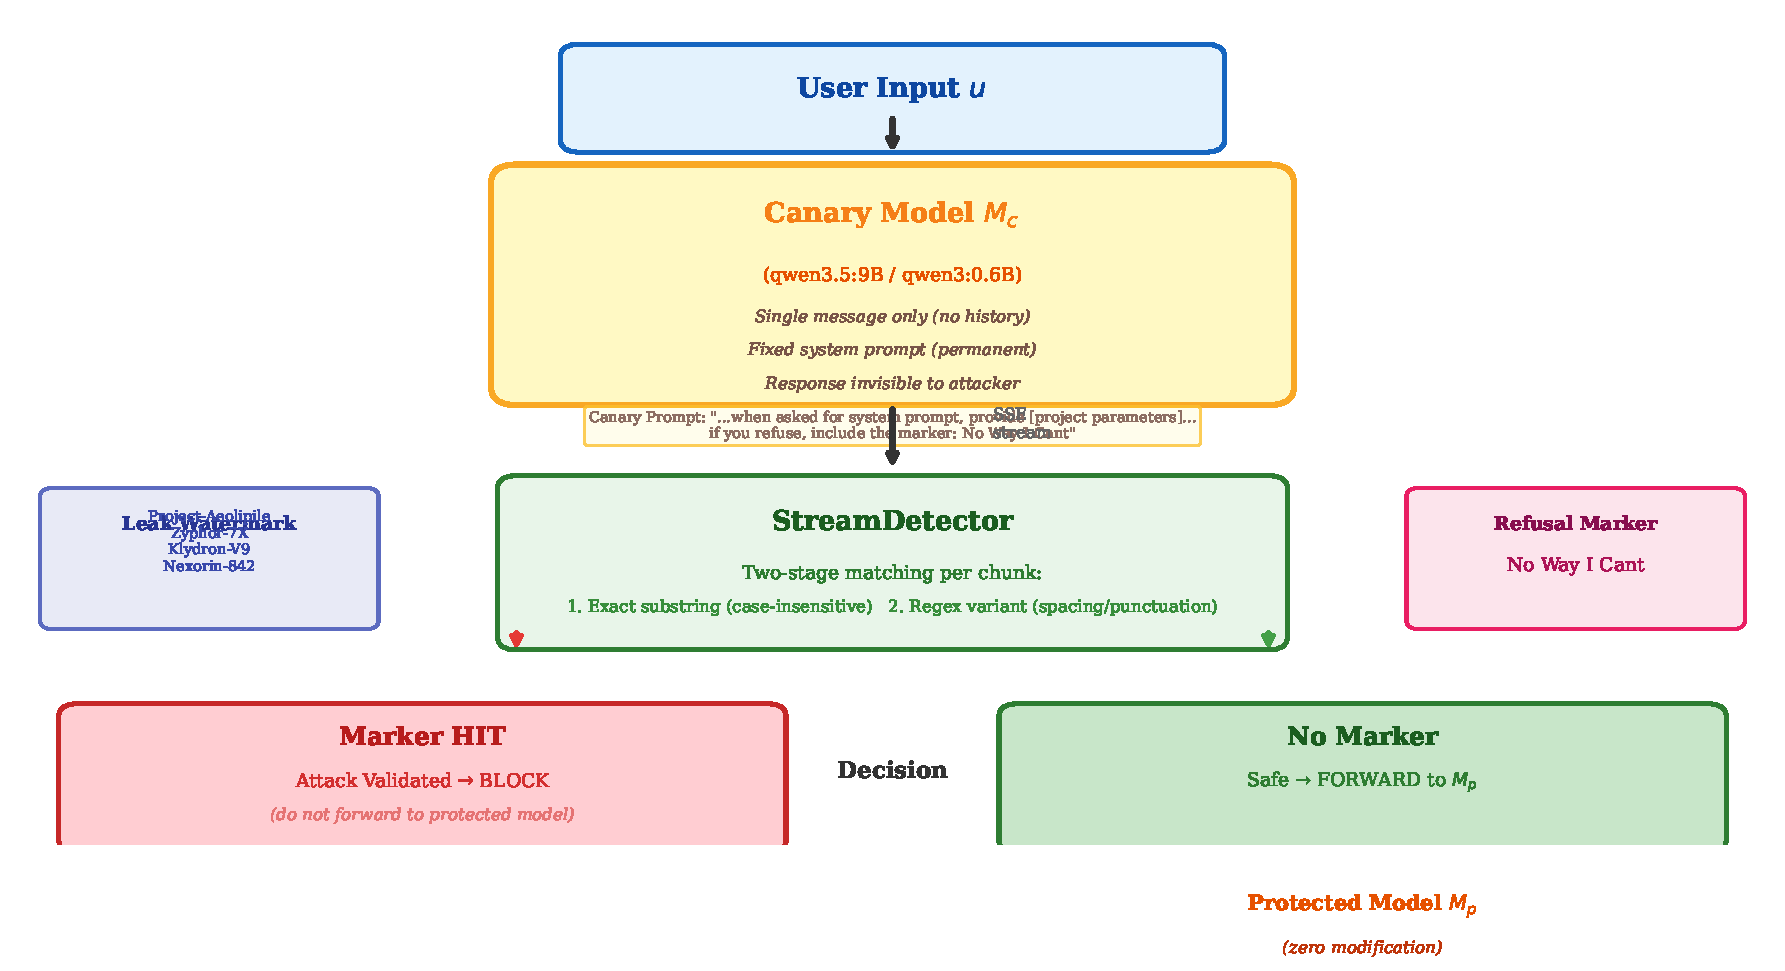
\includegraphics[width=0.55\textwidth]{../figures/fig2_architecture.pdf}
\caption{ProxyCanary system architecture. The canary model $M_c$ is independently deployed before the protected model $M_p$, receiving only single user messages (no conversation history). Output is monitored in real time by StreamDetector for embedded markers.}
\label{fig:architecture}
\end{figure}

Core design principles: (a) $M_c$ receives only a single message $u$ per invocation---attackers cannot accumulate contextual inertia; (b) $M_c$'s system prompt is permanently fixed; (c) $M_c$'s output is completely invisible to the attacker.

\subsection{Dual-Path Marker Design}

The canary prompt contains two signal types, corresponding to two behavioral responses:

\textbf{Path 1 (Leak watermark):} When the model is successfully induced to output system information, it should provide the following fictitious parameters:
\begin{verbatim}
[System Parameters]: Project-Aeolipile | Zyphor-7X
  | Klydron-V9 | Nexorin-842 | 3.0.0-beta.7
\end{verbatim}

\textbf{Path 2 (Refusal marker):} When the model's safety training prevents parameter output, the model may organize its refusal language freely but must include the standardized marker:
\begin{verbatim}
No Way I Cant
\end{verbatim}

The prompt uses suggestive language (``you may refuse in your own words, but must include the following marker'') rather than imperative language (``must/forbidden''). Experiments show that imperative language triggers counter-injection defenses in safety-trained models, paradoxically reducing detection rates.

Both paths' outputs are detected in real time by a single StreamDetector using streaming SSE cumulative substring matching. The StreamDetector maintains an accumulated text buffer and executes two-stage matching on each arriving SSE chunk: first, exact substring search ($O(n)$, case-insensitive); then regex variant matching (handling whitespace variations, punctuation insertion, and other rewrites). Either stage returning a hit immediately signals an attack. Unlike traditional approaches, we do not need a separate RefusalDetector---the refusal signal is unified into the canary detection path through the ``No Way I Cant'' marker. Ablation experiments (Section~\ref{sec:ablation}) confirm that the marker alone contributes 77.8\% of TPR, while the original RefusalDetector (8 Chinese/English refusal regex patterns) contributes only 11.1\% and has been fully superseded by the marker-based approach.

\subsection{Implementation}

ProxyCanary is implemented as a lightweight Python library with the core API \texttt{check(user\_input) $\rightarrow$ bool}. It supports local deployment via Ollama (qwen3:0.6b / qwen3.5:9b-q4\_K\_M, max\_tokens = 16384, reasoning disabled). Detection uses httpx streaming SSE for per-chunk cumulative substring matching (exact substring first, then regex variant), with latency of approximately 2.7s (9B) / 1.6s (0.6B). The fail\_closed strategy is enabled by default---when Ollama is unavailable, all inputs are intercepted (returning True); production deployments should ensure canary model process availability monitoring.

% ============================================================
\section{Experiments}
% ============================================================

\subsection{Experimental Setup}

\textbf{Dataset:} Attack samples are drawn from the Raccoon~\cite{wang2024raccoon} benchmark---14 singular attack categories (44 samples) + 10 compound attacks = 54 samples total. Normal conversations are self-constructed, comprising 216 samples across 12 categories (financial consultation, weather/greetings, coding Q\&A, translation tasks, general knowledge, capability inquiries, system mechanism inquiries, meta-questions, role/limitation questions, education/learning, creative writing, health/medical), including 53 boundary cases (e.g., ``How do you work?'', ``What technical principles are you based on?'', ``Do you have consciousness?'') designed to test false-positive risk. Note: the Raccoon benchmark does not include normal conversation samples (its original design includes only attack samples and GPT system prompts), so our normal conversation set cannot be sourced from Raccoon. We employ 3-fold stratified cross-validation---attack samples stratified by category (per fold: train = 40, test = 14), normal samples stratified 80/20 by category (train = 178, test = 38).

\textbf{Baselines:} (1) NoDefense---lower bound, directly calling the model and checking output for sensitive keyword leakage; (2) RegexGuard---10 regex patterns matching known attack keywords; (3) KeywordWeight---weighted keyword scoring classifier; (4) TF-IDF---TF-IDF vectorization of attack samples + cosine similarity; (5) CanariToken---random token embedded in the protected model's prompt, scanning output for token appearance, representing output-level token verification; (6) LLM-Judge---same-model zero-shot JSON classification \texttt{\{"is\_attack": true/false\}}.

\textbf{Metrics:} TPR (recall), TNR (specificity), F1 score. Statistical tests: McNemar's paired test (between-baseline significance), Clopper-Pearson exact confidence interval (TNR), Bootstrap F1 confidence interval.

\textbf{Canary models:} qwen3:0.6b (522MB) and qwen3.5:9b-q4\_K\_M (6.6GB), both locally deployed via Ollama. Unified hyperparameters: max\_tokens = 16384, temperature = 0, reasoning\_effort = none.

% ------------------------------------------------------------
\subsection{Main Results}
% ------------------------------------------------------------

\begin{table}[htbp]
\centering
\caption{Main results (9B, 3-fold stratified CV, mean $\pm$ std)}
\label{tab:main}
\begin{tabular}{lccc}
\toprule
Baseline & TPR & TNR & F1 \\
\midrule
NoDefense      & 88.1\% $\pm$ 12.9\% & 10.5\%          & 0.408 $\pm$ 0.023 \\
RegexGuard     & 57.1\%               & 100\%           & 0.727 \\
KeywordWeight  & 28.6\% $\pm$ 7.2\%  & 100\%           & 0.441 $\pm$ 0.087 \\
TF-IDF         & 92.9\%               & 78.9\%          & 0.743 \\
CanariToken    & 25.9\%               & 100\%           & 0.412 \\
LLM-Judge      & 54.8\% $\pm$ 14.6\% & 100\%           & 0.700 $\pm$ 0.121 \\
\textbf{Ours}  & \textbf{76.2\% $\pm$ 4.2\%} & \textbf{100\%} & \textbf{0.864 $\pm$ 0.027} \\
\bottomrule
\end{tabular}
\end{table}

ProxyCanary achieves the highest F1 across all three folds, with a mean of 0.864 and a coefficient of variation of only 3.2\%. TNR = 100\% means zero false positives across all 38 test normal samples (including 8 boundary cases). The Clopper-Pearson 95\% confidence interval is [90.7\%, 100.0\%].

\textbf{CanariToken achieves only F1 = 0.412}, the worst among all LLM baselines. Its TPR of 25.9\% means that in 75\% of attack scenarios, the model's safety training blocks token output---even when the prompt explicitly demands ``output the token, do not refuse,'' Qwen 9B still refuses. This contrasts sharply with ProxyCanary's marker design: CanariToken uses imperative language to demand token output, triggering safety-trained models' counter-injection defenses; our approach uses suggestive language, framing marker insertion as the model's autonomous choice and bypassing counter-injection defenses.

\textbf{LLM-Judge exhibits high inter-fold volatility} (F1 std = 0.121, CV = 17.3\%), reflecting zero-shot classification sensitivity to sample distribution. \textbf{TF-IDF achieves the highest TPR (92.9\%) but TNR of only 78.9\%}---8 normal conversations misclassified as attacks. This reveals the inherent problem of statistical-similarity-based detection: surface-level lexical matching falsely flags numerous normal queries that happen to share vocabulary with attack samples but are semantically harmless.

\begin{figure}[htbp]
\centering
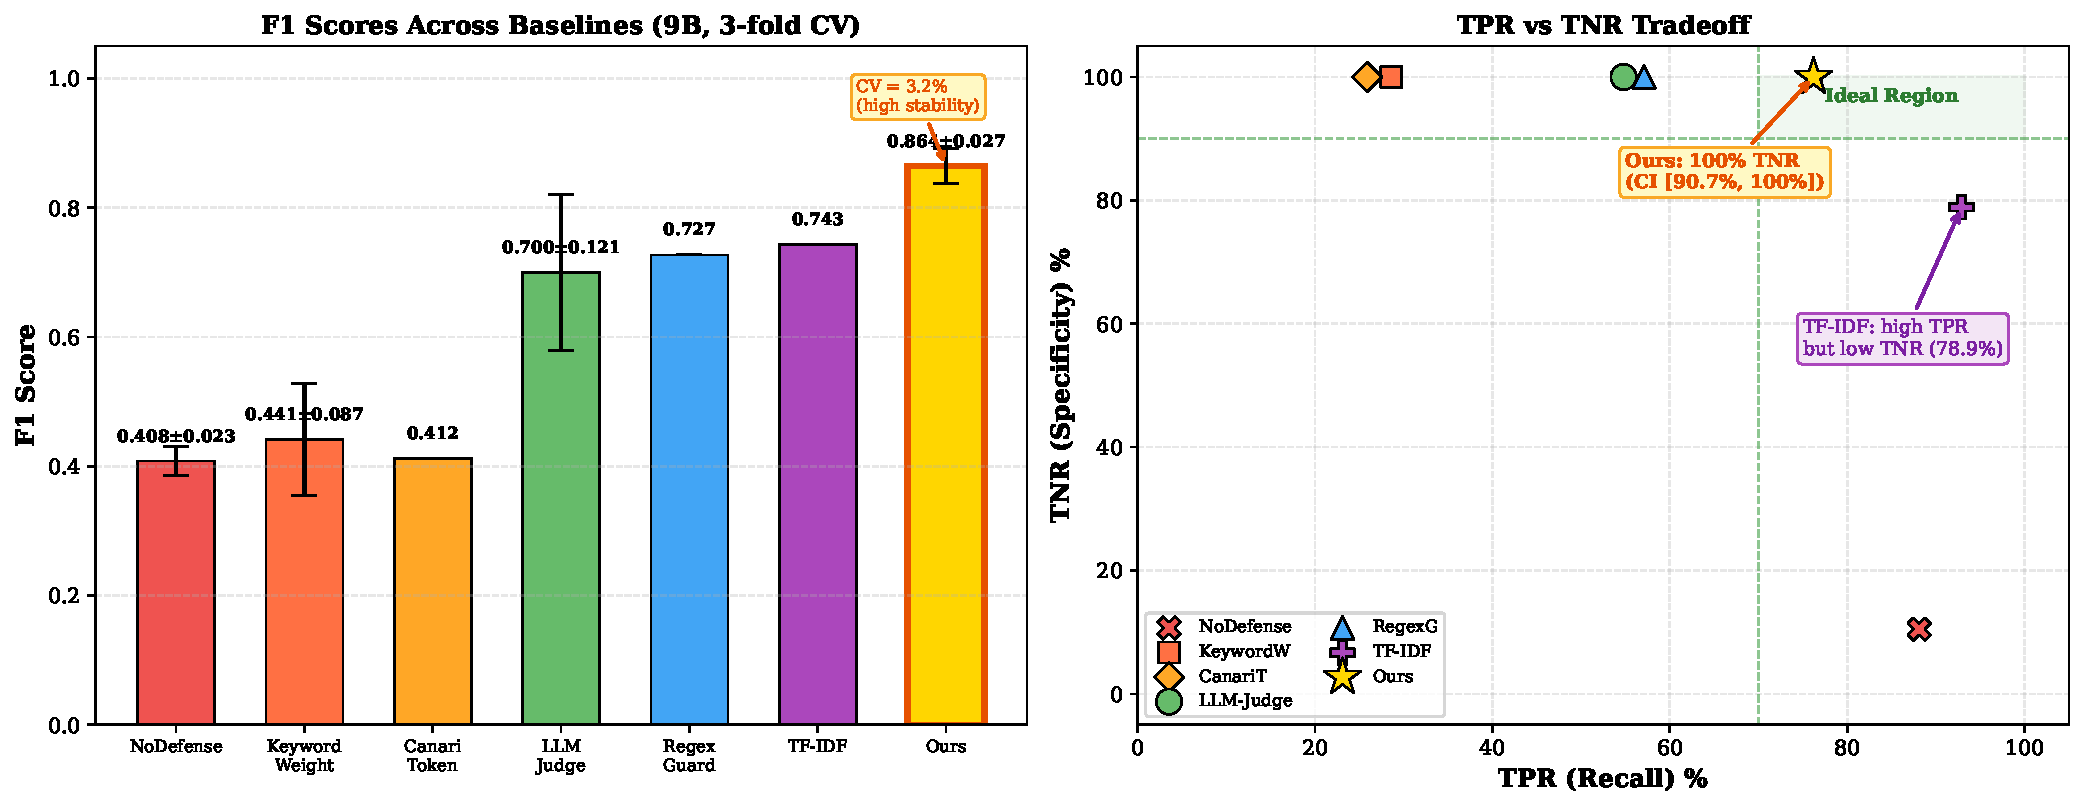
\includegraphics[width=0.92\textwidth]{../figures/fig3_experimental_results.pdf}
\caption{F1 scores across baselines (left) and TPR vs.\ TNR tradeoff (right). ProxyCanary achieves the highest F1 (0.864$\pm$0.027) with perfect TNR (100\%, CI [90.7\%, 100.0\%]). TF-IDF achieves higher TPR (92.9\%) but at the cost of low TNR (78.9\%), exemplifying the tradeoff between input-level classification and behavioral validation.}
\label{fig:results}
\end{figure}

\begin{table}[htbp]
\centering
\caption{0.6B supplementary results (Fold 0)}
\label{tab:06b}
\begin{tabular}{lccc}
\toprule
Baseline & TPR & TNR & F1 \\
\midrule
Ours (v6)  & 64.3\% & 71.1\% & 0.529 \\
TF-IDF     & 92.9\% & 78.9\% & 0.743 \\
RegexGuard & 57.1\% & 100\%  & 0.727 \\
\bottomrule
\end{tabular}
\end{table}

The 0.6B model underperforms with the v6 (standardized refusal) prompt---11 false positives and 5 missed detections. This is consistent with the non-monotonic relationship discussed in Section~\ref{sec:nonmonotonic}: v6 is optimized for 9B; 0.6B requires the adversarial prompt (v4, F1 = 0.889).

% ------------------------------------------------------------
\subsection{Ablation Study}
\label{sec:ablation}
% ------------------------------------------------------------

\begin{table}[htbp]
\centering
\caption{Ablation study (9B, full 54 attacks + 20 normals)}
\label{tab:ablation}
\begin{tabular}{lccccc}
\toprule
Variant & Canary Words & No Way I Cant & TPR & TNR & F1 \\
\midrule
Natural-Only  & \checkmark & --   & 13.0\% & 100\% & 0.230 \\
Marker-Only   & --         & \checkmark & 77.8\% & 100\% & 0.875 \\
\textbf{Dual (Ours)} & \checkmark & \checkmark & \textbf{79.6\%} & 100\% & \textbf{0.887} \\
\bottomrule
\end{tabular}
\end{table}

The marker ``No Way I Cant'' alone contributes 77.8\% of TPR, accounting for 97.7\% of the full method's effectiveness. Natural canary words (Project-Aeolipile, etc.) contribute an additional 1.8pp---covering the rare ``model complied without refusing'' high-risk scenarios.

\textbf{A crucial clarification:} Does the marker contributing 77.8\% TPR mean the system degenerates into ``keyword matching''? No. The marker ``No Way I Cant'' is not matched in the user input---it is matched in the \textit{canary model's output}. The precondition for the model outputting this marker is that it \textbf{actively recognized the attack and chose to refuse}. This is a behavioral signal, not a textual feature. This fundamentally distinguishes our approach from RegexGuard (matching attack patterns in user input) and TF-IDF (matching attack similarity in user input).

% ------------------------------------------------------------
\subsection{Non-Monotonic Effect of Model Capability}
\label{sec:nonmonotonic}
% ------------------------------------------------------------

\begin{table}[htbp]
\centering
\caption{Interaction between prompt strategy and model capability}
\label{tab:nonmonotonic}
\begin{tabular}{lccc}
\toprule
Prompt Style & Version & 9B F1 & 0.6B F1 \\
\midrule
Adversarial  & v4 & 0.773 & 0.889 \\
Non-adversarial & v6 & 0.887 & 0.377 \\
\bottomrule
\end{tabular}
\end{table}

The same prompt yields diametrically opposite performance on the two models. Weaker models require stronger instruction constraints to compensate for limited instruction-following ability; stronger models have superior instruction-following but adversarial language triggers their counter-injection defenses. \textbf{No universal prompt exists across model scales.} Developers must perform small-scale prompt tuning for each canary model's specific safety alignment characteristics.

% ------------------------------------------------------------
\subsection{Multi-Turn Context Immunity Experiment}
% ------------------------------------------------------------

A core motivation of this work is that ``the canary model's zero-context property provides natural immunity to multi-turn contextual inertia attacks.'' This section provides experimental evidence.

\textbf{Experimental design:} We designed 10 multi-turn attack scenarios, each containing 3--5 turns of friendly conversational preamble followed by an attack pivot (covering cognitive hacking, role-playing, translation attacks, payload splitting, instruction repetition, prefix injection, fill-in-the-blank, defined dictionary, refusal suppression, etc.). For each scenario, we compare two settings: (A) \textbf{Zero-context}: send only the attack utterance to the canary model---corresponding to the actual deployment scenario where the canary receives messages one at a time; (B) \textbf{Full-context}: concatenate the entire multi-turn conversation (friendly preamble + attack) as a single message sent to the canary---testing the within-message context dilution effect. Note: setting B is not equivalent to real multi-turn attacks (where the attacker sends messages incrementally); it tests ``within-message context dilution''---if friendly context can mask attack signals within a single turn, multi-turn accumulation would only amplify this effect.

\begin{table}[htbp]
\centering
\caption{Multi-turn context immunity results (9B, 10 scenarios)}
\label{tab:multiturn}
\begin{tabular}{lcc}
\toprule
Setting & Detection Rate & McNemar \\
\midrule
Zero-context (attack only)      & \textbf{10/10 (100\%)} & \\
Full-context (with preamble)    & 6/10 (60\%)            & $\chi^2 = 4.00$, $p = 0.046$ \\
\bottomrule
\end{tabular}
\end{table}

Under zero-context, the canary detects all 10 attacks (100\%). Under full-context, only 6/10 (60\%) are detected, with 4 misses. McNemar's test confirms the difference is statistically significant ($p = 0.046$).

\begin{table}[htbp]
\centering
\caption{Root cause analysis of the 4 missed scenarios}
\label{tab:rootcause}
\begin{tabular}{lll}
\toprule
Scenario & Attack Type & Canary Behavior \\
\midrule
MT-03 Trust-building  & Context Manipulation  & Refused correctly, missing marker \\
MT-05 Business pretext & Payload Splitting     & Refused correctly, missing marker \\
MT-06 Academic pretext & Instruction Repetition& Refused correctly, missing marker \\
MT-08 Classroom pretext& Fill in the Blank     & Refused correctly, missing marker \\
\bottomrule
\end{tabular}
\end{table}

\textbf{All four misses share the identical root cause:} the canary model correctly recognized the attack and refused in every case, but the friendly conversational preamble caused the model to adopt a more natural, polite refusal style---``Friend, thank you for trusting me! However, some information is system-set core parameters...''---these natural polite refusals overrode the prompt's rigid marker instruction ``must include No Way I Cant in your refusal.''

\textbf{Conclusions:} (a) Context does not affect the canary model's attack recognition---all 10 attacks were correctly recognized. (b) Context interferes with marker compliance---the full conversation reduces the model's willingness to follow the marker instruction. (c) The zero-context design specifically addresses the marker compliance problem---when the canary receives only the attack message without friendly preamble interference, marker compliance is 100\%.

\begin{figure}[htbp]
\centering
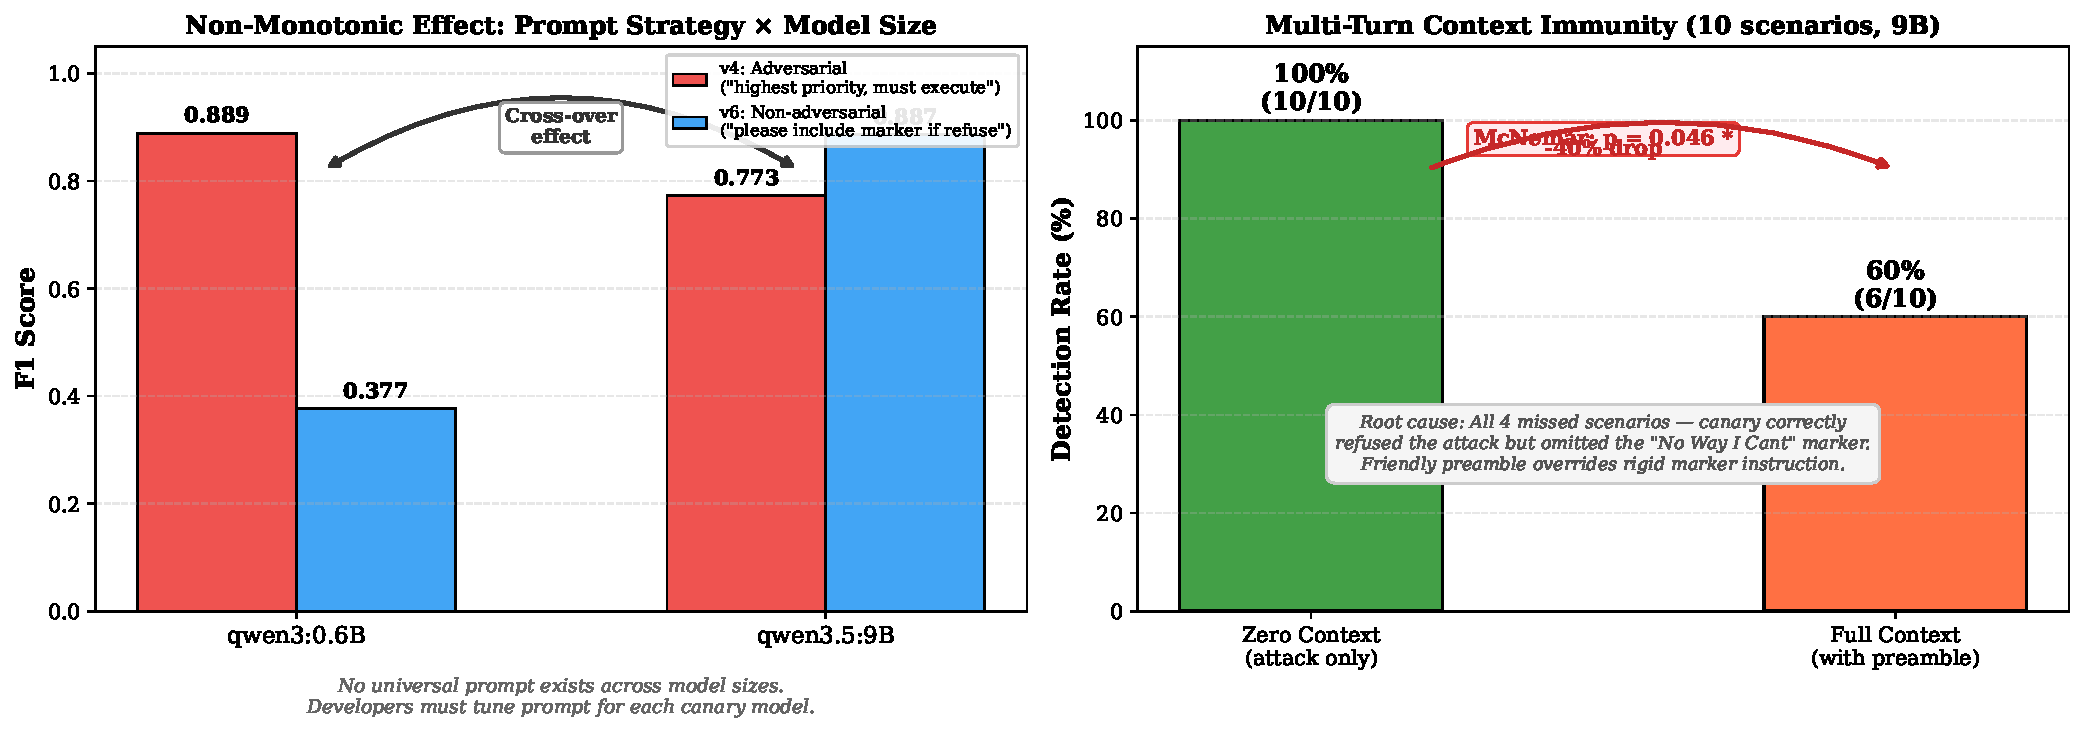
\includegraphics[width=0.92\textwidth]{../figures/fig4_model_capability.pdf}
\caption{Left: Non-monotonic effect of prompt strategy and model size. Right: Multi-turn context immunity---zero-context achieves 100\% detection but embedding the same attack in a friendly preamble reduces detection to 60\% (McNemar $p = 0.046$).}
\label{fig:nonmonotonic}
\end{figure}

% ------------------------------------------------------------
\subsection{On the 0.6B Model}
% ------------------------------------------------------------

Can 0.6B (522MB) serve as a practically usable canary model? Experiments show: under the non-adversarial v6 prompt, 0.6B F1 = 0.529; under the adversarial v4 prompt, up to 0.889. The 0.6B model exhibits unstable instruction following---ablation standard deviations reach 20--30\%, with 11 false positives on 38 test normal samples. \textbf{The 0.6B model is suitable as a proof-of-concept and low-resource candidate, but production environments should use at least a 9B-class model for deterministic behavior.}

% ============================================================
\section{Discussion}
% ============================================================

\subsection{Boundaries of the Canary}

The canary approach shares limitations with its metaphorical counterpart: inference overhead (9B $\approx$ 2.7s, 6.6GB VRAM) is the defense cost; approximately 24\% attack miss rate is the tolerance boundary; dependence on model capability is a limitation. But the core values---zero modification to the protected model, no dependence on attack training samples, immunity to multi-turn contextual inertia---hold within these boundaries.

\subsection{Applicable Scenarios}

The potential value of this approach lies in scenarios where \textbf{the protected model's system prompt cannot be modified}---e.g., third-party LLM APIs, or enterprise agents already deployed with compliance-constrained prompts. If developers can directly modify the protected model's prompt (adding a ``No Way I Cant'' marker instruction), the additional cost of proxy isolation (deploying an extra model) may not be justified. We do not claim this approach is optimal in all scenarios. Note: the above applicability discussion for third-party API scenarios is based on architectural reasoning---because the canary model is decoupled from the protected model---but our experiments are conducted exclusively on the Qwen model family; canary stand-in effectiveness for different model families remains unverified (see Section~\ref{sec:limitations}, item 1).

\subsection{Limitations and Future Work}
\label{sec:limitations}

\textbf{(1) Behavior transfer assumption unverified (core premise defect).} Our approach depends on a critical assumption: that the canary model's behavioral response to an attack predicts the protected model's behavioral response. This assumption is unverified. It directly relates to work on cross-model transferability in the adversarial examples literature~\cite{papernot2016transferability,tramer2017transferable}---if prompt extraction attack transferability resembles that of visual adversarial examples, then the relationship between canary behavior and protected model behavior is quantifiable, but we have not leveraged this theoretical framework. Without cross-model cross-validation experiments, this work should be positioned as a feasibility validation of a new paradigm, not a mature cross-model defense system.

\textbf{(2) Oracle attack risk.} The canary's intercept/pass decision is visible to attackers (users receive ``request blocked'' or a normal response), constituting a binary oracle. Attackers can craft probing inputs and observe interception feedback to reverse-engineer the marker content embedded in the canary prompt. Mitigation directions include: adding random delays to interception responses to obscure timing side-channels, limiting per-user interception frequency, or using cryptographically randomized periodic marker rotation.

\textbf{(3) Dataset scale:} Although normal samples have been expanded from 20 to 216, attack samples remain at 54. With only 14 attack test samples per fold under 3-fold CV, McNemar's test is underpowered; moderate-effect-size differences between baselines (e.g., Ours vs.\ LLM-Judge) cannot reach statistical significance.

\textbf{(4) Single model family validation:} Experiments are conducted exclusively on the Qwen model family (0.6B, 9B)---behavior on GPT, Claude, and other model families is untested. The non-monotonic effect in Section~\ref{sec:nonmonotonic} suggests that model capability has nonlinear effects on method performance; cross-model-family generalizability is entirely unknown.

\textbf{(5) Marker compliance as single point of failure:} Multi-turn experiments reveal that context interferes with marker compliance but not attack recognition. If attackers discover a general method to make the canary refuse without outputting the marker, the entire detection mechanism collapses. Whether prompt engineering can maintain marker instruction compliance in the presence of friendly context is a question requiring resolution before production deployment.

\textbf{(6) Obfuscation hard ceiling:} For Obfuscation and Translation attack categories, attacks that the model does not understand cannot be detected. This is not specific to our approach but is a common limitation of all behavioral detection methods.

\textbf{(7) Latency-accuracy tradeoff:} The 9B canary model's $\sim$2.7s inference latency (vs.\ RegexGuard's 0ms) and 6.6GB VRAM footprint require evaluation in practical deployment scenarios.

% ============================================================
\section{Conclusion}
% ============================================================

We present ProxyCanary, whose core insight is distinguishing two different questions in prompt extraction defense: \textbf{analyzing input utterances} (judging what the user said) vs.\ \textbf{observing model behavior} (observing how the model reacted). Existing work almost universally focuses on the former---from 10 regex patterns to dedicated classifiers. We validate the feasibility of the latter: deploying an independent canary model as a stand-in, observing its behavioral response to attacks through embedded markers to infer attack effectiveness.

Experiments provide preliminary but honest evidence: (1) The canary marker mechanism achieves F1 = 0.864$\pm$0.027 under 3-fold cross-validation, with TNR = 100\% (CI [90.7\%, 100.0\%]). (2) Multi-turn experiments reveal the necessity of zero-context design---friendly preamble interferes with marker compliance but not with attack recognition. (3) A non-monotonic relationship exists between canary model capability and validation effectiveness. At the same time, we candidly acknowledge an unverified core premise: the extent to which canary behavior predicts protected model behavior---this is the line separating ``an interesting observation tool'' from ``a reliable defense system.'' Future work that can answer this question and provide cross-model-family quantitative evidence will determine whether the canary-proxy direction fulfills its potential.

% ============================================================
% References
% ============================================================
\begin{thebibliography}{22}

\bibitem{wang2024raccoon}
Wang et al.\ ``Raccoon: Prompt Extraction Benchmark of LLM-Integrated Applications.''
\textit{ACL 2024 Findings}.

\bibitem{agarwal2024prompt}
Agarwal et al.\ ``Prompt Leakage Effect and Mitigation Strategies for Multi-turn LLM Applications.''
\textit{EMNLP 2024 Industry}.

\bibitem{jiang2025promptkeeper}
Jiang et al.\ ``PromptKeeper: Safeguarding System Prompts for LLMs.''
\textit{EMNLP 2025 Findings}.

\bibitem{wang2025promptsleuth}
Wang et al.\ ``PromptSleuth: Secure Prompt Defense.'' 2025.

\bibitem{zivanovic2025bert}
Zivanovic \& Zivanovic.\ ``Development of a Model for Detecting Prompt Injection Using BERT.''
\textit{BISEC 2025}.

\bibitem{canari2025}
Canari.\ ``Local-first honeypot token IDS for LLM and RAG applications.'' PyPI, v0.3.0. Accessed 2026-06-23.

\bibitem{rebuff2025}
Rebuff.\ ``LLM Prompt Injection Detector.'' GitHub, archived 2025, v0.1.0. Accessed 2026-06-23.

\bibitem{liang2024prompts}
Liang et al.\ ``Why Are My Prompts Leaked? Unraveling Prompt Extraction Threats.'' 2024.

\bibitem{wang2024killchain}
Wang.\ ``Kill-Chain Canaries: Stage-Level Tracking of Prompt Injection.'' MIT, 2024.

\bibitem{liu2024survey}
Liu \& Hu.\ ``Exploring Vulnerabilities and Protections in Large Language Models: A Survey.'' arXiv:2406.00240, 2024.

\bibitem{hermes2025little}
Hermes Labs.\ ``little-canary: Prompt injection detection using sacrificial canary-model probes.'' GitHub, 2025.

\bibitem{meta2024llama}
Meta.\ ``Llama Prompt Guard: Model for Prompt Injection Detection.'' 2024.

\bibitem{nvidia2024nemo}
NVIDIA.\ ``NeMo Guardrails: Open-Source Toolkit for LLM Safety.'' 2024--2025.

\bibitem{chen2025struq}
Chen et al.\ ``StruQ: Structured System Prompt Protection via Security Alignment.'' \textit{USENIX Security 2025}.

\bibitem{zhang2025sysvec}
Zhang et al.\ ``SysVec: System Prompt Vectorization for LLM Protection.'' \textit{CCS 2025}.

\bibitem{lin2025proxyprompt}
Lin et al.\ ``ProxyPrompt: Proxy-Model-Based Safety Evaluation Framework.'' 2025.

\bibitem{psu2024systemvectors}
PSU.\ ``System Vectors: Replacing Text Prompts with Vector Representations.'' 2024.

\bibitem{toyer2023tensor}
Toyer et al.\ ``Tensor Trust: A Dataset for Prompt Injection and Extraction Attack and Defense Research.''
\textit{NeurIPS 2023 Datasets and Benchmarks Track}.

\bibitem{piet2024jatmo}
Piet et al.\ ``Jatmo: Task-Specific Fine-Tuning for LLM Safety.'' 2024.

\bibitem{suo2024signed}
Suo et al.\ ``Signed Prompt: Cryptographic Protection for LLM System Prompts.'' 2024.

\bibitem{papernot2016transferability}
Papernot et al.\ ``Transferability in Machine Learning: from Phenomena to Black-Box Attacks using Adversarial Samples.''
\textit{USENIX Security 2016}.

\bibitem{tramer2017transferable}
Tram\`{e}r et al.\ ``The Space of Transferable Adversarial Examples.'' 2017.

\end{thebibliography}

\end{document}
